\section{Conclusion}
	\begin{itemize}
			\item \todo{We need a coordination at the language level, explicit by using a dedicated language and that enables the verification and validation of the coordinated system}
			
			\item \todo{The knowledge about system integration is currently either implicitly held by the integrator or encoded within a framework. To capture explicitly this knowledge and thus leverage integrator know-how, we propose a dedicated language to capture coordination patterns between languages, thus reifying the coordination specification at the language level.}
	\end{itemize}


         	\begin{figure}
         		\begin{center}
         			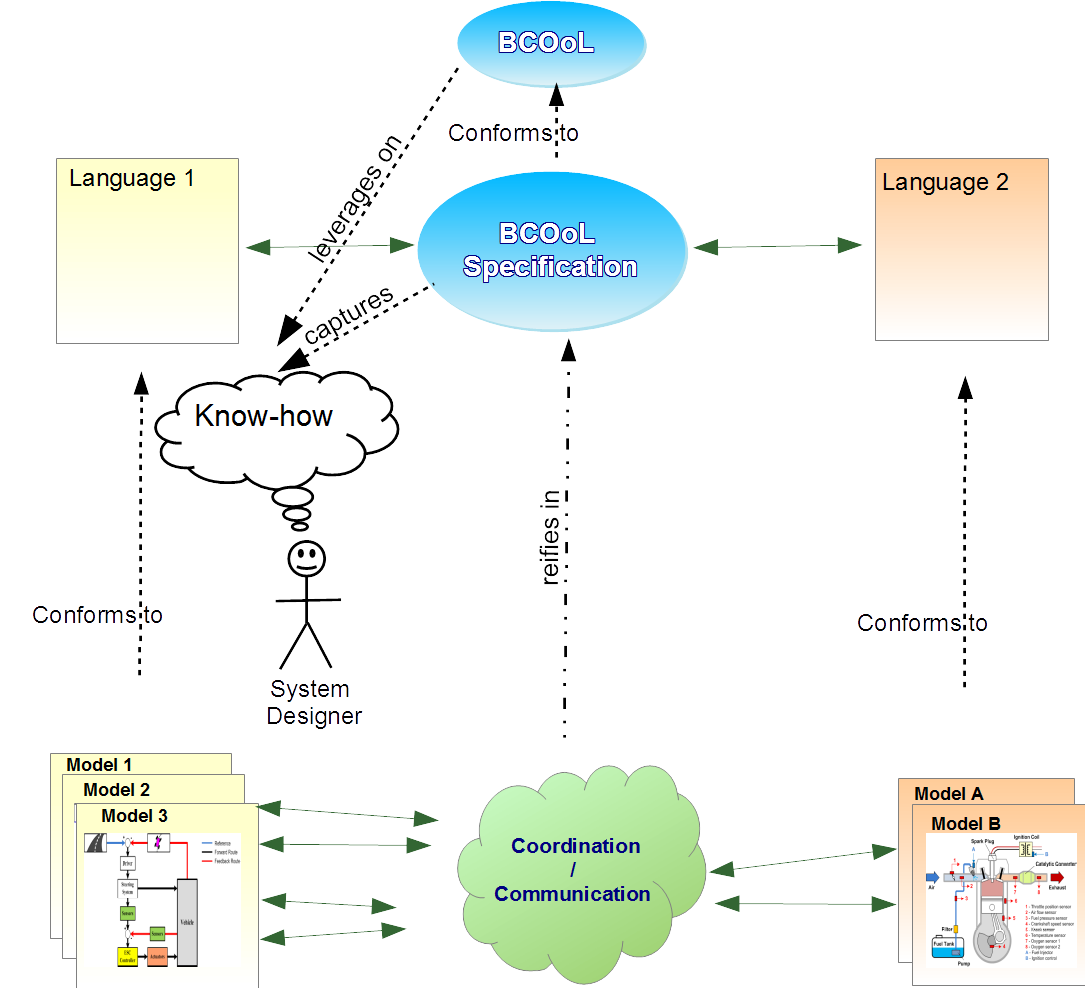
\includegraphics[width=0.7\textwidth]{background/figs/bcoolapp.png}
         			\caption{Overview of Our Approach}
         			\label{fig:diNatale}
         		\end{center}
         	\end{figure}	

\begin{table}[h]
	\centering
	\caption{Overview of state of art approaches}
	\label{my-label}
	\begin{tabular}{cccccc}
		\multicolumn{1}{l}{\multirow{2}{*}{Approach}} & \multicolumn{1}{l}{\multirow{2}{*}{Syntactic Composition}} & \multicolumn{2}{c}{Semantics Composition} & \multirow{2}{*}{Specification} & \multirow{2}{*}{Application} \\
		\multicolumn{1}{l}{}                          & \multicolumn{1}{l}{}                                       & Composition         & Coordination        &                                &                              \\
		Epsilon                                       & Yes                                                        &                     &                     & Lenguage Level                 & Model Level                  \\
		Ptolemy\cite{ptoleframebib}                                      & No                                                         &                     & X                   & Language Level                 & Model Level                  \\
		Rapide                                        & No                                                         &                     & X                   & Model Level                    & Model Level                  \\
		Esper                                         & No                                                         &                     & X                   & Model Level                    & Model Level                  \\
		MASCOT                                        & No                                                         &                     & X                   & Language Level                 & Model Level                  \\
		\cite{compostatechartsbib}                  & No                                                         & X                   &                     & Language Level                 & Model Level                      
	\end{tabular}
			\todo{To use one page and put all studied approaches}
\end{table}